\documentclass{article}
\author{Lena Morrill}
\date{\today}
\title{Transcriptomic analysis of the organoids}

\usepackage{tikz}
\usepackage{lscape}
\usepackage{array}
\usepackage{graphicx}
\usepackage{hyperref}

\setlength{\textwidth}{6.7in}
\setlength{\oddsidemargin}{-0.1in}
\setlength{\textheight}{8.6in}
\setlength{\topmargin}{-0.4in}

\def\checkmark{\tikz\fill[scale=0.4](0,.35) -- (.25,0) -- (1,.7) -- (.25,.15) -- cycle;} 
\newcolumntype{L}[1]{>{\raggedright\let\newline\\\arraybackslash\hspace{0pt}}m{#1}}
\newcolumntype{C}[1]{>{\centering\let\newline\\\arraybackslash\hspace{0pt}}m{#1}}
\newcolumntype{R}[1]{>{\raggedleft\let\newline\\\arraybackslash\hspace{0pt}}m{#1}}


\begin{document}
\maketitle

\tableofcontents

\section{Data}
\subsection{3' bias}

Three RNASeq samples -- PDO14, PDO16, and PDO18 -- have a clear 3' bias. Three others -- PDO4, PDO13, PDO17 -- have a slighy bias. Only the first three have been removed from the analysis.

\subsection{Summary of organoids}

% latex table generated in R 4.0.3 by xtable 1.8-4 package
% Fri Mar 12 11:30:34 2021

\begin{landscape}

\begin{table}[ht]
{ \scriptsize
\centering
\begin{tabular}{rL{.4in}L{.3in}L{.3in}L{.3in}R{.3in}L{.1in}L{.1in}L{.3in}llL{.2in}L{.3in}L{.2in}L{.3in}L{.15in}L{.15in}L{.2in}L{.2in}L{.2in}L{.3in}L{.3in}L{.3in}}
  \hline
 & PDO & ID & sWGS & RNAseq & OVO4& & Cor. CN-GE & Comments & scDNA? & S4 & WGD & CCNE1 amp & CCNE1 amp (RNA or CN) & Chromotripsis & Tandem dup & \#segments & Ploidy & Quiet & Change from ascites & CDK12 amp & CDK12 loss & Chemonaive \\ 
  \hline
1 & PDO1 & 151723 & 19844 & 19938 & 920.00 &  & Y & Very similar to PDO11 &  & \checkmark & \checkmark &  &  &  &  & Very low & Very high &  & ? & $\times$ & $\times$ & \checkmark \\ 
  2 & PDO11 & 54327 & 118976 & 19905 & 413.00 &  & N & Very similar to PDO1 &  &  & &  & \checkmark &  &  & Very low & Med &  & $\times$ & $\times$ & $\times$ & $\times$ \\ 
  3 & PDO10 & 119178 & 119127 & 19907 & 788.00 &  & N &  &  & \checkmark &  &  &  &  &  & Med & Med &  & ? & $\times$ & $\times$ & $\times$ \\ 
  4 & PDO13 & 54276 & 19846 & 19940 & 297.00 &  & Y &  &  &  &  &  &  &  &  & Med & Med &  & ? & \checkmark & $\times$ & $\times$ \\ 
  5 & PDO15 & 118947 & 54327 & 19904 & 333.00 &  & N &  &  & \checkmark &  &  &  &  &  & Med & Med &  & $\times$ & $\times$ & $\times$ & $\times$ \\ 
  6 & PDO17 & 50495 & 50495- & 19916 & 348.00 &  & Y &  &  & \checkmark &  &  &  &  &  & Med & Med &  & ? & $\times$ & $\times$ & $\times$ \\ 
  7 & PDO18 & 32070 & 32070- & 19920 & 47.00 &  & - &  &  & \checkmark &  &  &  &  &  & Low & Med &  & ? & $\times$ & $\times$ & $\times$ \\ 
  8 & PDO2 & 23868 & jb95a- & 19917 & 75.00 &  & Y &  & \checkmark & \checkmark &  & \checkmark & \checkmark &  &  & Med & Med &  & ? & $\times$ & $\times$ & $\times$ \\ 
  9 & PDO3 & 118976 & 119178 & 19906 & 466.00 &  & N &  & \checkmark & \checkmark &  &  & \checkmark & \checkmark &  & Med & Med &  & $\times$ & $\times$ & $\times$ & $\times$ \\ 
  10 & PDO9 & 119058 & 119058- & 19921 & 466.00 &  & Y &  &  & \checkmark &  &  &  & (!) surely also has tandem duplication? &  & Med & Med &  & ? & $\times$ & $\times$ & $\times$ \\ 
  11 & PDO14 & 54288 & 19829 & 19925 & 409.00 &  & - &  &  & \checkmark &  &  & \checkmark &  &  & High & Med &  & $\times$ & \checkmark & $\times$ & $\times$ \\ 
  12 & PDO4 & 151773 & 19848 & 19942 & 571.00 &  & Y &  &  & \checkmark &  &  & \checkmark &  & \checkmark & Very high & Med &  & ? & $\times$ & $\times$ & $\times$ \\ 
  13 & PDO5 & 119127 & 118947 & 19903 & 627.00 &  & N &  &  & \checkmark &  &  &  &  &  & Med & Med &  & ? & $\times$ & $\times$ & $\times$ \\ 
  14 & PDO6 & 119148 & 119148 & 19902 & 627.00 &  & Y &  & \checkmark & \checkmark &  &  &  &  &  & Med & Med &  & ? & $\times$ & $\times$ & $\times$ \\ 
  15 & PDO16 & 119025 & 19842 & 19936 & 839.00 &  & - &  &  &  &  &  &  &  &  & Low & Low & \checkmark & $\times$ & $\times$ & \checkmark & $\times$ \\ 
  16 & PDO12 & 151761 & 19845 & 19939 & 467.00 &  & Y &  &  &  &  &  &  &  &  & Low & Low & \checkmark & \checkmark & $\times$ & \checkmark & $\times$ \\ 
  17 & PDO7 & 32077 & 19847 & 19941 & 366.00 &  & Y &  &  &  &  &  &  &  &  & Low & Low & \checkmark & ? & $\times$ & $\times$ & $\times$ \\ 
  18 & PDO8 & 54059 & 19843 & 19937 & 366.00 &  & Y &  &  &  &  &  &  &  &  & Low & Low & \checkmark & ? & $\times$ & $\times$ & $\times$ \\ 
%  19 & FT1 & fal01 &  & 19950 &  &  &  &  &  &  &  &  &  &  &  &  &  &  &  &  &  &  \\ 
%  20 & FT10 & fal10 &  & 19953 &  &  &  &  &  &  &  &  &  &  &  &  &  &  &  &  &  &  \\ 
%  21 & FT7 & fal07 &  & 19952 &  &  &  &  &  &  &  &  &  &  &  &  &  &  &  &  &  &  \\ 
%  22 & FT7-bis & fal07 &  & 19954 &  &  &  &  &  &  &  &  &  &  &  &  &  &  &  &  &  &  \\ 
%  23 & FT8 & fal08 &  & 19955 &  &  &  &  &  &  &  &  &  &  &  &  &  &  &  &  &  &  \\ 
%  24 & FT9 & fal09 &  & 19951 &  &  &  &  &  &  &  &  &  &  &  &  &  &  &  &  &  &  \\ 
   \hline
\end{tabular}
}
\end{table}

\end{landscape}

\section{Transcriptomics of organoids}

\begin{figure}[h]
\centering
\includegraphics[width=3.2in]{../../RNASeq_DE_resistant_sensitive/figures/PCA_RNASeq/3primebias_PCA_counts.pdf}
\includegraphics[width=3.4in]{../../RNASeq_DE_resistant_sensitive/figures/PCA_RNASeq/PCA_counts_subset_BRCA_TAMSeq.png}
\caption{PCA including all samples (left) and only the ones without 3' bias (right; colour coded by number of mutations in BRCA.)}
\end{figure}

\subsection{Organoids $vs$ normal ovarian tissue DE}

\begin{center} \emph{Done by Stephane} \end{center}

\subsection{Sensitive organoids $vs$ resistant organoids DE}
\begin{center} \emph{Done by Stephane} \end{center}


\clearpage
\subsection{Comparison with TCGA}

\begin{figure}[h]
\centering
\includegraphics[width=.42\textwidth]{../../RNASeq_DE_resistant_sensitive/figures/Sensitive_resistant_figures/colmeans_deseqcounts_correlation_tcga_org.pdf}
\includegraphics[width=\textwidth]{../../RNASeq_DE_resistant_sensitive/figures/Sensitive_resistant_figures/TPM_correlation_tcga_org_selected_genes.pdf}
\caption{TPM for genes of interest in organoids (points) and in TCGA (violin plots). Genes which have a different distribution according to a Kolmogorov-Smirnov test are marked with an asterisk.}
\end{figure}

\clearpage

\subsection{(Resistant $vs$ sensitive in organoids) $vs$ (complete remission or response $vs$ progressive disease in TCGA) }

Extremely bad correlation for both log2 fold changes and $p$ values. As we don't expect to find a perfect match anyway (as (1) progressive disease would work as a surrogate for resistant, but there are many more factors and (2) it's an organoid comparison $vs$ a primary tissue comparison) we have left this on standby.

\section{Correlation of gene expression and copy number}

There are two values for gene expression that we can work with:
\begin{itemize}
\item (Computed by Lena) the weighted average copy number value per gene
\item (Computed by Stephane) the copy number value is assigned to each gene which is the closest to a copy number area of high variability (variability computed with the variance across samples)
\end{itemize}

In the genes of interest (MYC, etc.) the two are almost always the same (meaning that the relevant copy number segment is on the gene). The conclusions from Stephane's analysis is that there were some correlations in certain genes, but that it was mostly driven by only a couple of organoids (!). There were some extreme copy number values that were excluded as outliers -- they all belong to the samples 118976org or 119058org, that come from the same patient.

There is no obvious correlation between raw CN values and counts (TPM or DESeq2), either pooling all organoids or doing an organoid-specific scatterplot (See Figures \href{https://github.com/lm687/Organoids_Compositional_Analysis/blob/master/RNASeq_and_CN/figures/joint_counts_CN_DESeq_all.pdf}{[scatterplot per organoid DESeq2]} and \href{https://github.com/lm687/Organoids_Compositional_Analysis/blob/master/RNASeq_and_CN/figures/joint_counts_CN_TPM_all.pdf}{[scatterplot per organoid TPM]}).

\medskip

This prompted us to scale the CN and GE values (scaled between organoids to a mean of zero and a standard deviation of 1). This gives a much better correlation, especially when segments of copy number of two are excluded from the analysis (see \ref{fig:scaled_CN_GE}). However, it seems as though this trend only applies to some organoids. Organoids PDO11, PDO10, PDO15, PDO3, PDO5 show no trend between GE and CN. These organoids don't have anything special when it comes to exposures, and they are not the ones with relatively high 3' bias.

\medskip

A similar approach is to compare the ranks of the organoids in CN and GE (see Figure~\ref{fig:rank_CN_GE}).

\medskip

A couple of important considerations: gene expression values are correlated (only slightly, but this can become important in whole genome analyses), and copy number regions can be extremely large, making the link between copy number and any gene very tenuous.

\begin{figure}[h]
\centering
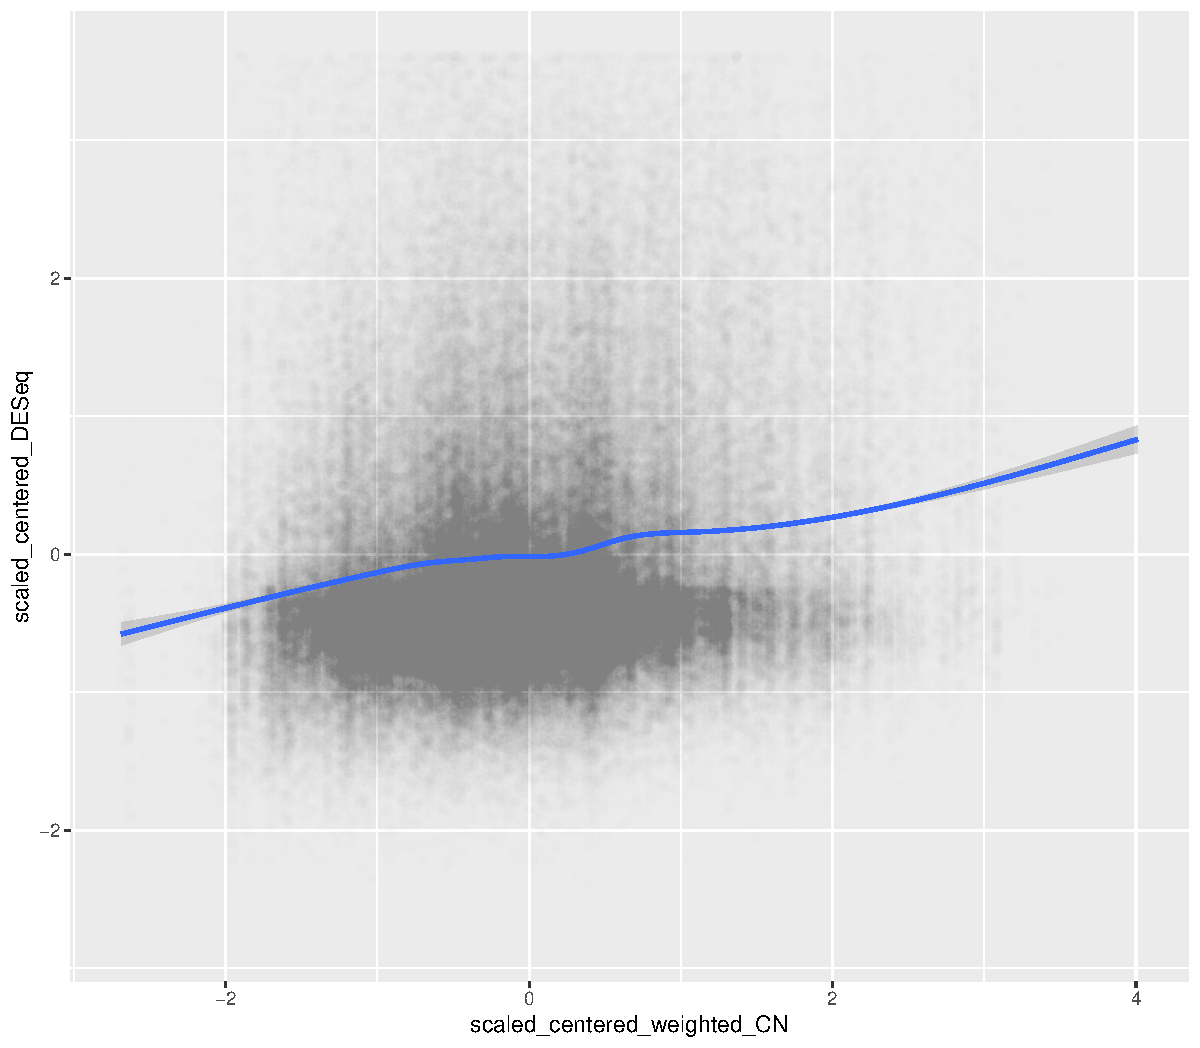
\includegraphics[width=1.7in]{../../RNASeq_and_CN/figures/scatterplot_normCNweighted_normDESeq_nonormal.png}
\includegraphics[width=1.7in]{../../RNASeq_and_CN/figures/scatterplot_normCNweighted_normTPM_nonormal.png}
\includegraphics[width=2.8in]{../../RNASeq_and_CN/figures/scatterplot_normCNweighted_normDESeq_perorg2_subsetorgs.png}\\
\includegraphics[width=\textwidth]{../../RNASeq_and_CN/figures/scatterplot_normCNweighted_normDESeq_perorg2.png}
%\includegraphics[width=1.7in]{../../RNASeq_and_CN/figures/scatterplot_normCNweighted_normDESeq_nonormal_onlyamp.png}
\caption{Scaled and centered CN and GE (DESeq2 and TPM respectively). Below: split per organoid. The same results are found when normal segments are kept. \label{fig:scaled_CN_GE}} %When only looking at amplifications (third plot; for DESeq2 counts) the trend is even clearer}
\end{figure}


\begin{figure}[h]
\centering
\includegraphics[width=3in]{../../RNASeq_and_CN/figures/rankplot_CNweighted_deseq.pdf}
\caption{Relative abundances of agreement of ranks between GE and CN, for all genes. A brighter diagonal indicates a very good agreement in the rank of GE and rank of CN across organoids.\label{fig:rank_CN_GE}}
\end{figure}

\medskip

If we ask the question of whether genes which are in highly amplified regions have a higher gene expression than the same gene in normal fallopian tissue (average over five fallopian samples of healthy patients) the answer is overwhelmingly \emph{not} (102174 sample/genes combinations for which it's not the case,  64621 for which it is, when the copy number is higher than 2), with most genes having actually lower expression values than normal tissue. This is confounded by compositionality/ assuming that most genes remain the same. This includes most genes of interest.

\begin{figure}[h]
\centering
\includegraphics[width=.45\textwidth]{../../RNASeq_and_CN/figures/CN_violinplots_goi.pdf}
\includegraphics[width=.45\textwidth]{../../RNASeq_and_CN/figures/CN_violinplots_goi_2.pdf}
\includegraphics[width=3in]{../../RNASeq_and_CN/figures/r2normCNnormDESeq_vs_averagebottomCN.pdf}
\includegraphics[width=3in]{../../RNASeq_and_CN/figures/r2normCNnormDESeq_vs_averagebottomCN_best.pdf}
\includegraphics[width=2.5in]{../../RNASeq_and_CN/figures/example_KRT6B.pdf}
\includegraphics[width=3in]{../../RNASeq_and_CN/figures/average_bottomCN_DESeq.pdf}
\caption{Fraction of samples with gene expression higher than the bottom three samples of lowest copy number. Higher values indicate a correlation between copy number and gene expression.}
\end{figure}

\end{document}